\chapter{Evidencias del prototipo}
\label{cap:anexog}

\section*{G.1. Alcance}

Este anexo reúne únicamente las capturas indispensables para comprender el flujo del
demostrador: entrada del incidente, entrada de voz experimental, recomendación
interpretable y registro de la decisión humana. Las pantallas proceden de una ejecución
local con casos sintéticos y no contienen datos personales ni información operativa
real del servicio 112.

Las capturas acreditan la existencia de una interfaz funcional, pero no sustituyen la
evaluación cuantitativa del Capítulo~\ref{cap:9} ni constituyen una prueba de usabilidad
con operadores profesionales.

\section*{G.2. Entrada del incidente}

La Figura~\ref{fig:g-entrada} muestra el formulario empleado para introducir un caso
controlado. El texto y los campos auxiliares se revisan antes de ejecutar la cadena de
inferencia.

\begin{figure}[htbp]
    \centering
    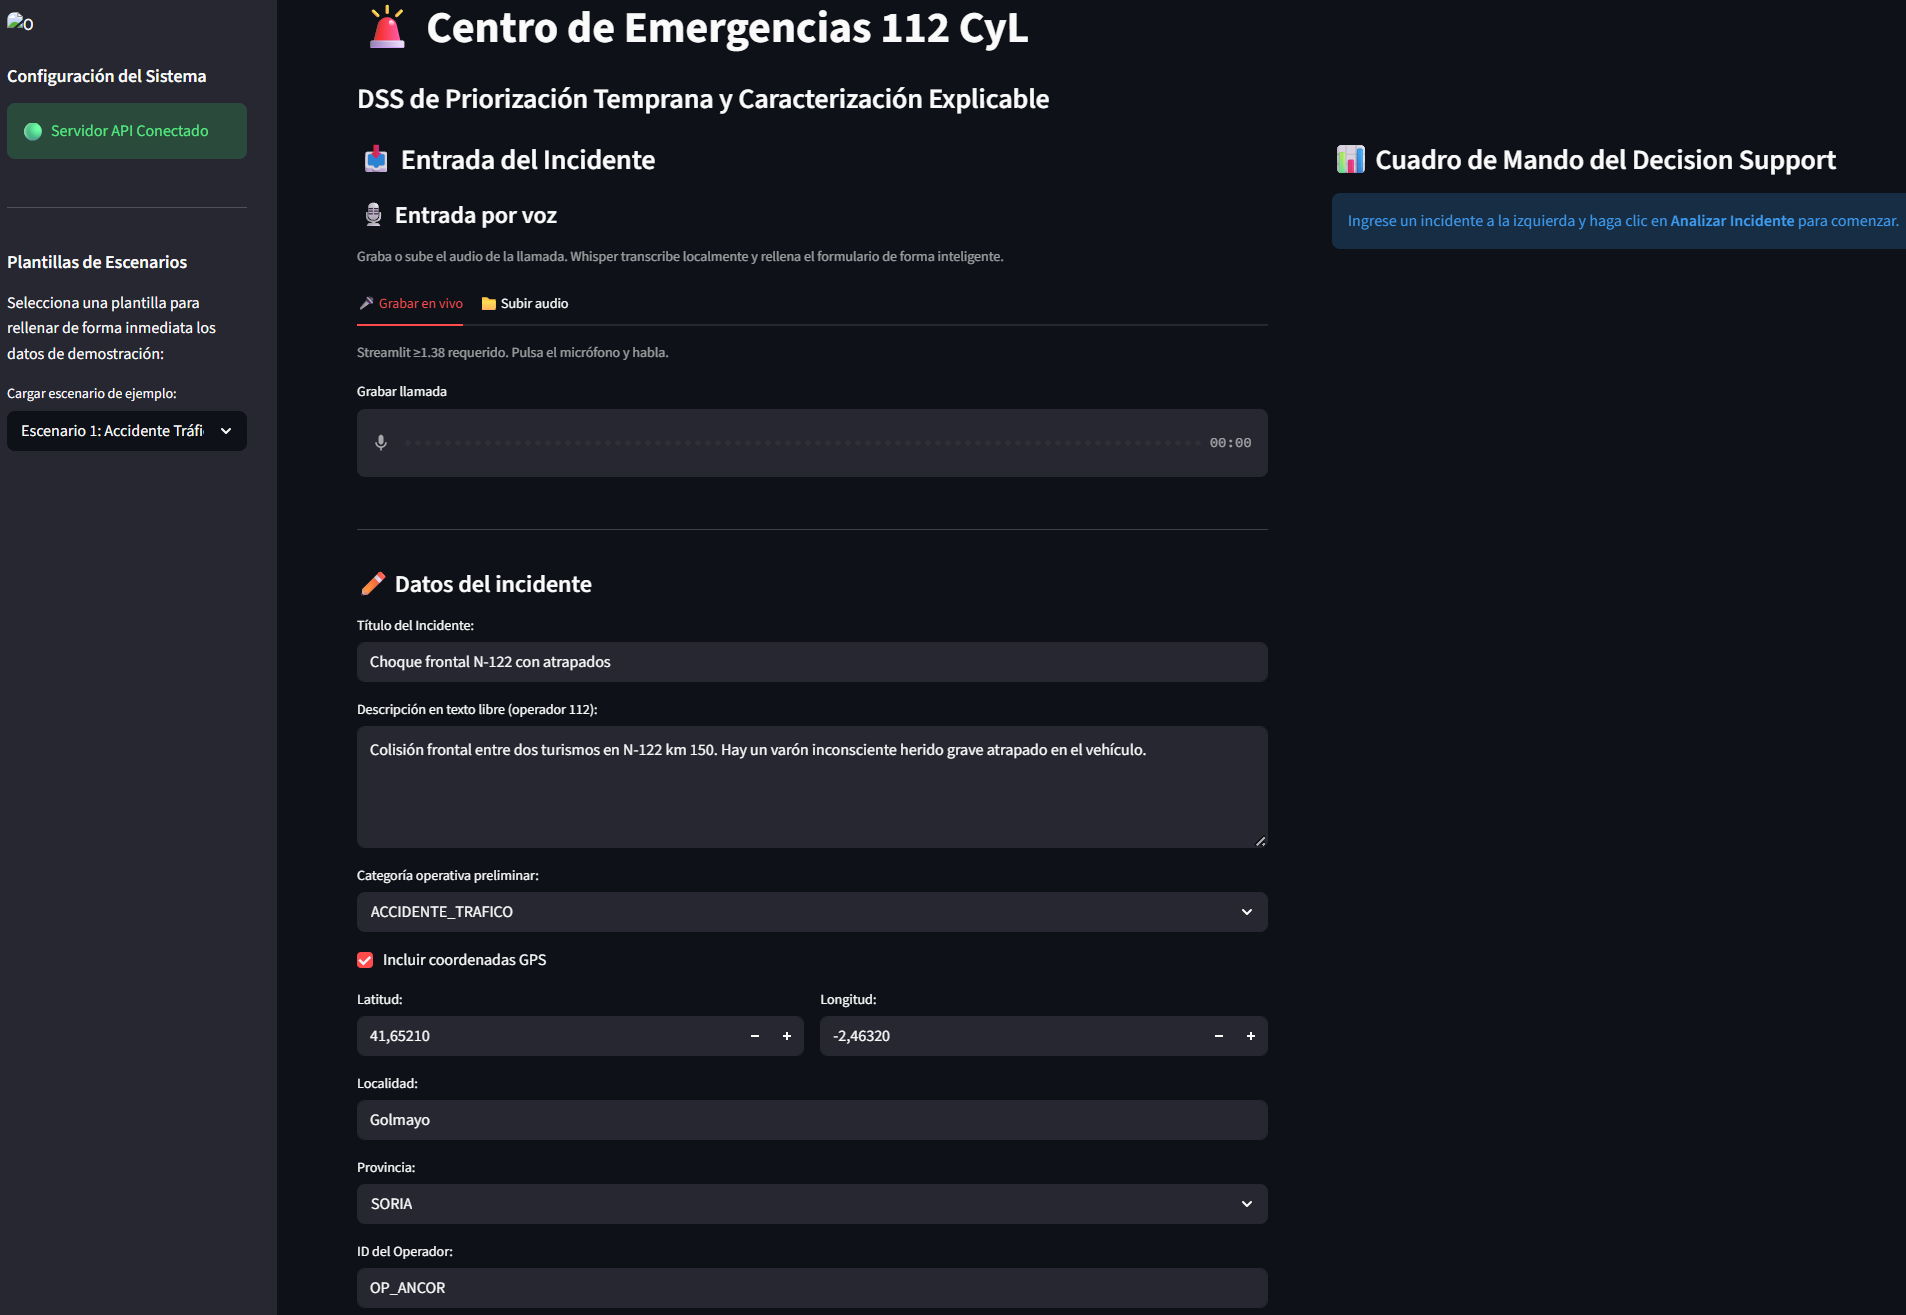
\includegraphics[width=0.88\textwidth]{figures/prototype_v0_1_0/g01_entrada_incidente.png}
    \caption{Entrada manual de un incidente sintético en la interfaz del prototipo.}
    \label{fig:g-entrada}
\end{figure}

\section*{G.3. Entrada de voz experimental}

El módulo de reconocimiento automático del habla (ASR) permite grabar o cargar audio de
prueba y proponer una transcripción para completar el formulario. La persona usuaria
debe revisar y corregir el resultado antes de solicitar una recomendación. Esta
funcionalidad es experimental y no ha sido validada con llamadas reales, ruido de sala
ni locutores representativos.

\begin{figure}[htbp]
    \centering
    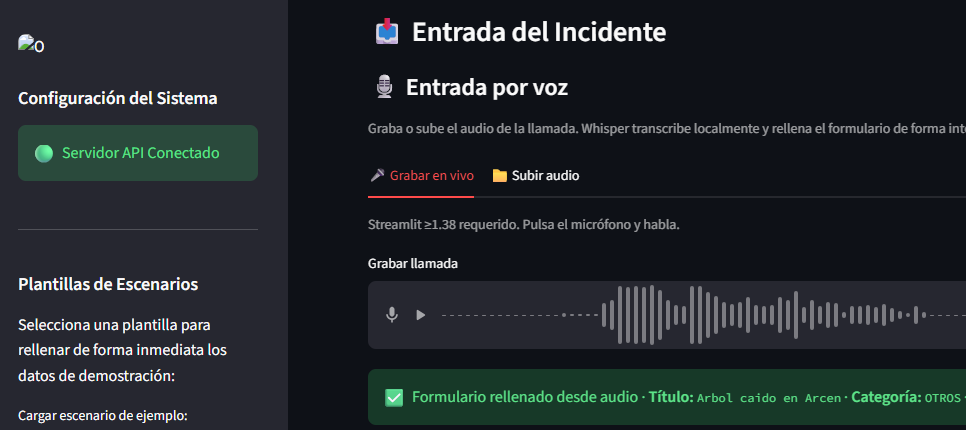
\includegraphics[width=0.82\textwidth]{figures/prototype_v0_1_0/g02_entrada_voz.png}
    \caption{Módulo experimental de entrada por voz mediante \texttt{faster-whisper}.}
    \label{fig:g-voz}
\end{figure}

\section*{G.4. Recomendación interpretable}

La Figura~\ref{fig:g-p1} recoge las dos partes de la salida para un escenario P1. La
interfaz separa la recomendación y distribución de probabilidades de Capa 2 de la
explicación generada por Capa 3. El modelo de lenguaje no modifica la prioridad.

\begin{figure}[htbp]
    \centering
    \begin{minipage}[t]{0.49\textwidth}
        \centering
        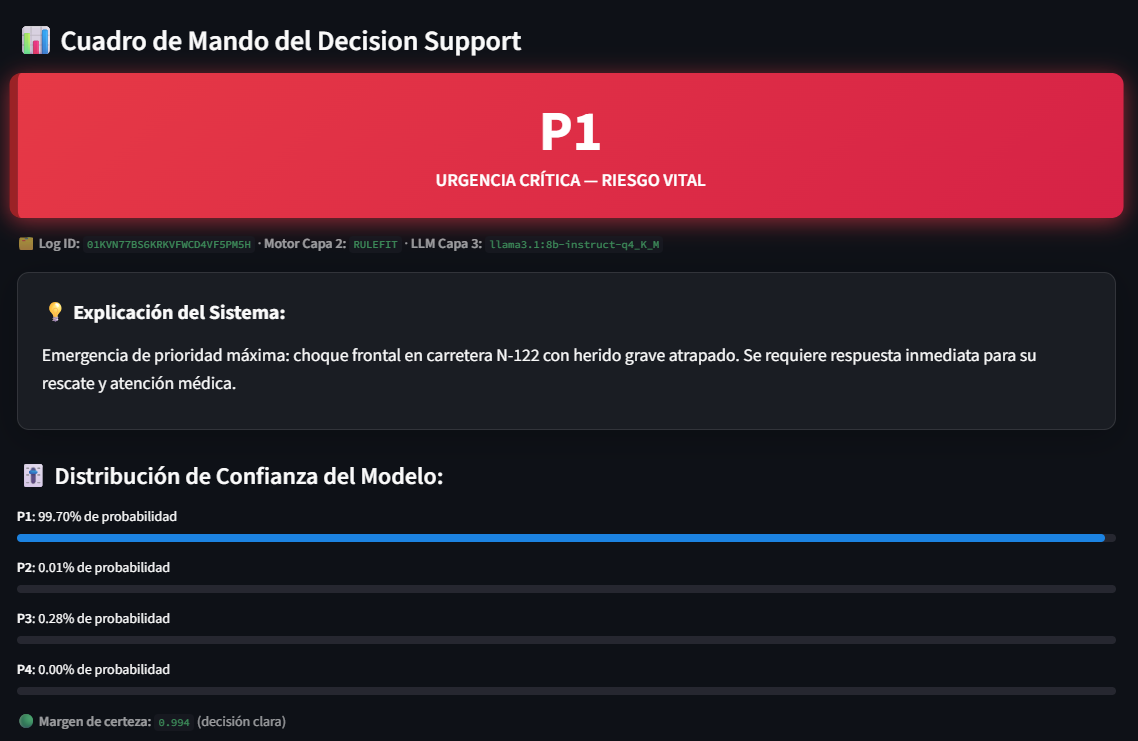
\includegraphics[width=\linewidth]{figures/prototype_v0_1_0/g03_resultado_p1_a.png}
        \small (a) Prioridad y probabilidades.
    \end{minipage}
    \hfill
    \begin{minipage}[t]{0.49\textwidth}
        \centering
        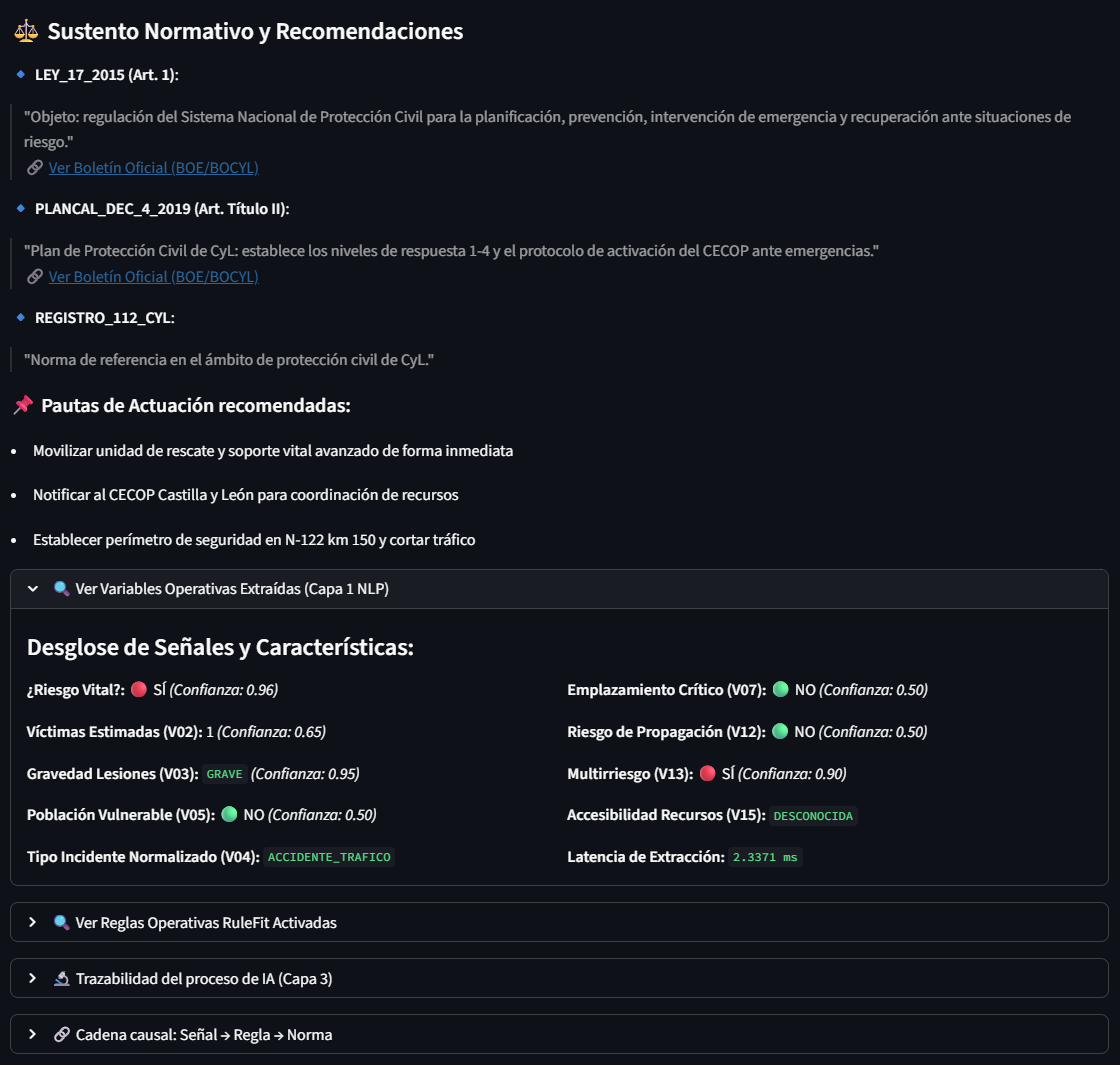
\includegraphics[width=\linewidth]{figures/prototype_v0_1_0/g03_resultado_p1_b.png}
        \small (b) Reglas, explicación y contexto.
    \end{minipage}
    \caption{Resultado de un incidente sintético clasificado como P1.}
    \label{fig:g-p1}
\end{figure}

\section*{G.5. Registro de la decisión humana}

La última evidencia muestra el formulario de retroalimentación. Su finalidad es
registrar si la recomendación se acepta, modifica o rechaza y conservar la justificación
correspondiente. La muestra de 119 casos fue revisada cualitativamente y de forma conjunta
por los tres autores; el formulario queda disponible para una futura evaluación
independiente y trazable, sin que la revisión interna equivalga a validación externa.

\begin{figure}[htbp]
    \centering
    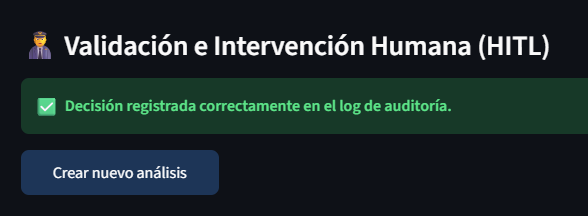
\includegraphics[width=0.72\textwidth]{figures/prototype_v0_1_0/g06_feedback_humano.png}
    \caption{Formulario para registrar la decisión humana y una posible discrepancia.}
    \label{fig:g-feedback}
\end{figure}
